\input{style/settings}
\input{style/short_commands}
\pagestyle{fancy}
\fancyhf{}
\fancyhead[R]{página\;\thepage/\pageref{LastPage}}
\fancyhead[L]{Osvaldo Uriel Calderón Dorantes}
\fancyfoot[L]{Imagenología Biomédica}
\fancyfoot[R]{Facultad de Ciencias, UNAM 
\includegraphics[scale=0.13]{style/Sheikah.pdf}}
\fancypagestyle{plain}{
  \fancyfoot[C]{}
}
\makeatletter
\def\@seccntformat#1{%
  \expandafter\ifx\csname c@#1\endcsname\c@section\else
  \csname the#1\endcsname\quad
  \fi}
\makeatother
%%%%%%%%%%%%%%%%%%%%%%%%%%%%%%%%%%%%%%%%%%%%%%%%%%%%%%%
%%%%%%%%%%%%%%%%%%%%%%%%%%%%%%%%%%%%%%%%%%%%%%%%%%%%%%%%%%%
\begin{document}
\begin{flushleft}
Osvaldo Uriel Calderón Dorantes, \hfill Imagenología Biomédica\\
316005171 \hfill osvaldo13576@ciencias.unam  \\
Facultad de Ciencias\\
\underline{Universidad Nacional Autónoma de México}
\end{flushleft}

\begin{flushright}\vspace{-5mm}

\includegraphics[height=1.5cm]{style/logo.pdf}
\end{flushright}
 
\begin{center}\vspace{-1cm}
\textbf{ \large \customfont{Examen 2\\
Módulo RADIODIAGNÓSTICO}}\\
\today
\end{center}
%\medskip\hrule\medskip
%%%%%%%%%%%%%%%%%%%%%%%%%%%%%%%%%%%%%%%%%%%%%%%%
%{\small \textbf{Nota: A las unidades las pondré dentro de corchetes \ec{[\tx{unidad}]} para no confundir entre variables y realizar el análisis dimensional fácilmente.}}
\medskip\hrule\bigskip

\newlength{\strutheight}
\settoheight{\strutheight}{\strut}


\begin{enumerate}[1.]
\item  Menciona las primeras cuatro generaciones de tomógrafos con sus respectivas características. Dibuje un esquema de cada uno.


        \begin{figure}[!ht]
          \centering
          \subfigure[]{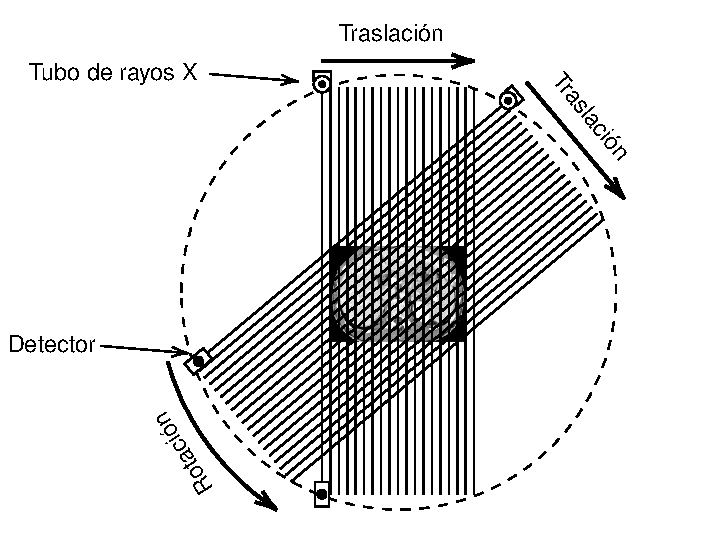
\includegraphics[width=0.45\textwidth]{./figuras/ct_1gen.pdf}} 
          \subfigure[]{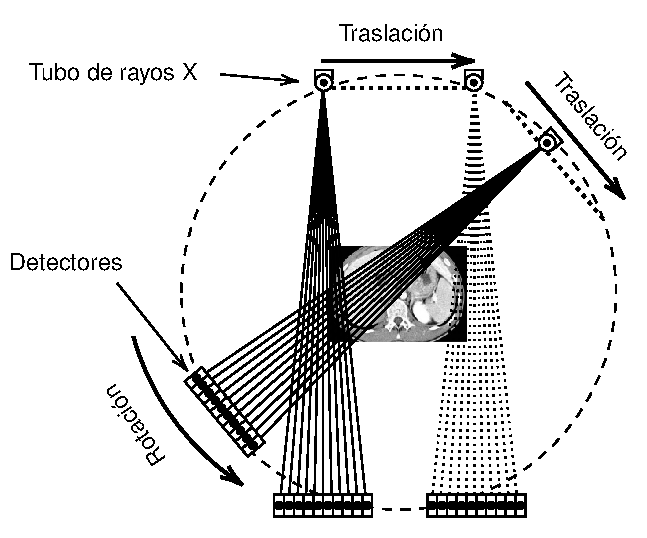
\includegraphics[width=0.45\textwidth]{./figuras/ct_2gen.pdf}} 
          \subfigure[]{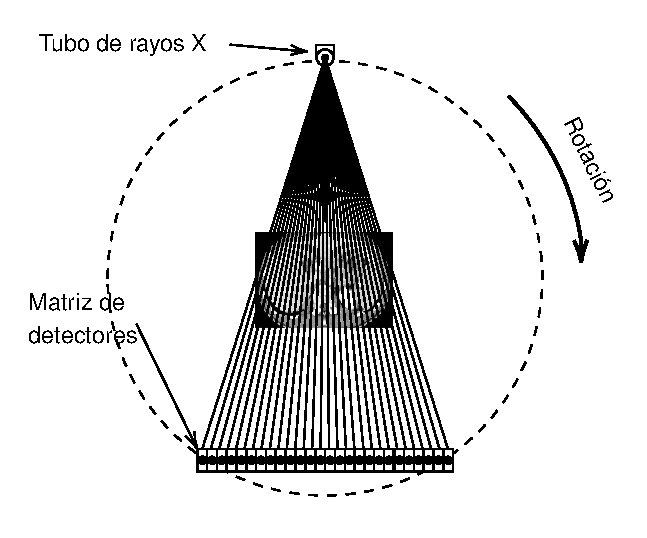
\includegraphics[width=0.45\textwidth]{./figuras/ct_3gen.pdf}}
          \subfigure[]{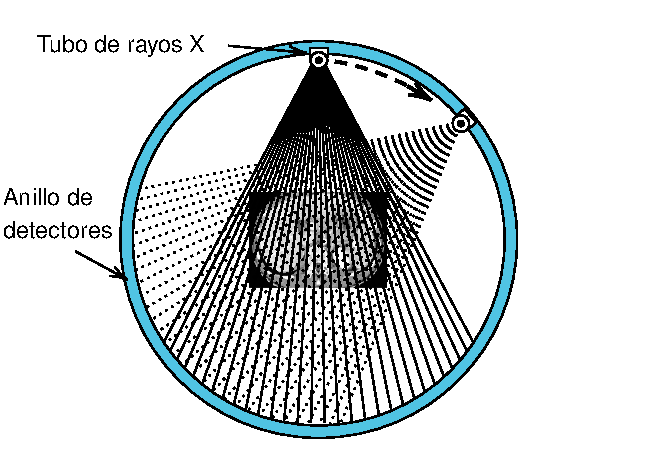
\includegraphics[width=0.45\textwidth]{./figuras/ct_4gen.pdf}}
          \caption{(a) CT primera generación (b) CT segunda generación (c) CT tercera generación (d) CT cuarta generación}
          \label{fig:CT}
      \end{figure}
     
En la figura \ref{fig:CT} se puede observar los esquemas de los tomógrafos de la primera, segunda, tercera y cuarta generación. A continuación se muestran las características de éstos:


\begin{enumerate}[(a)]
  \item \textbf{Primera generación}: En esta primera generación se empleaba un haz de rayo X de geometría de lápiz el cual se colimaba para tener esa forma, su movimiento consistía en una combinación de movimiento de traslación y rotación, dentro del sistema, el tubo de rayos X y el detector se encontraban en posiciones opuestas y dispuestos colinealmente, cada exploración se realizada grado por grado y tomaba cerca de 160 muestras por cada grado por lo que era una adquisición lenta y, además no tenía buena resolución espacial y tenía bajo contraste.
  \item \textbf{Segunda generación}: En la segunda generación se empleó un haz con forma de abanico angosto de hasta \ec{10^\circ} y múltiples detectores que consistía en un arreglo lineal de 30 detectores, en cada rotación el sistema hacía un paso de \ec{10^\circ}, sin embargo, este sistema requería un sistema mecánico sumamente preciso para obtener buenas imágenes.
  \item \textbf{Tercera generación}: El sistema del tubo y detector ahora en cada movimiento solo era de rotación, en lugar de realizar la traslación en cada paso, el haz con forma de abanico se sigue conservando, también cuenta con una serie de detectores del ancho del haz de entrada.
  \item \textbf{Cuarta generación}: En esta generación se incorpora una serie de haz que abarca todo el sistema de manera circular y dispuesto de manera estacionaria, ahora el tubo de rayos X es el que rota alrededor del paciente dando un haz de geometría de abanico.
\end{enumerate}



\item ¿En qué consiste la CT helicoidal?

\begin{figure}[!ht]
  \center
  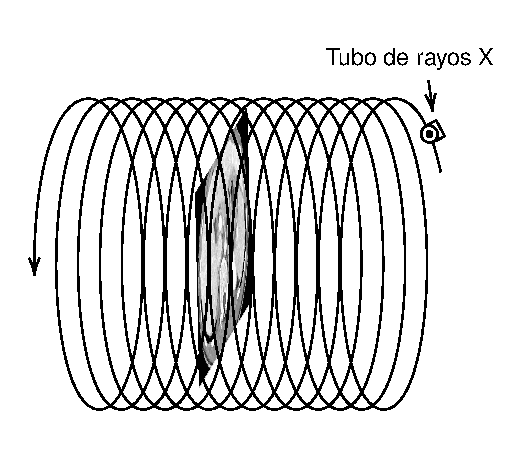
\includegraphics[scale=0.8]{./figuras/heli.pdf}
  \caption{Esquema de CT helicoidal.}
  \label{fig:p2}
  \end{figure}

En la CT helicoidal la adquisición de datos consiste en que el paciente se mueve a lo largo del eje horizontal conforme el tubo de ratos X se mueve alrededor del paciente en forma de hélice, como se muestra en la figura \ref{fig:p2}. La reconstrucción de la imagen consiste en el uso de la interpolación de los datos de la proyección a lo largo del eje del paciente en una región de interés y es posible usar los algoritmos de reconstrucción en donde gracias a la interpolación se puede suponer que el haz de rayos X se mueve de manera circular y no de manera helicoidal.

\item ¿Qué es la ecualización del histograma?

Consiste en un método para imágenes en donde se realiza un ajuste al contraste de la imagen digital de tal manera que la distribución de tonos de grises por pixel sea el mismo, es decir, este proceso distribuye de manera uniforme las intensidades por pixel.

\item ¿ En qué consisten las técnicas algebraicas y de retroproyección?


\begin{itemize}
  \item \textbf{Algebraicas}:  Esta técnica consiste en asignar un valor a cada pixel de la imagen digital de acuerdo al coeficiente de atenuación en esa región, entonces dado que el cuerpo no es un material uniforme, así que el haz de rayo X será atenuado que atraviesa por cierta región, por lo que la ley de atenuación exponencial queda como \ec{I=I_0\exp\p{-\sum_{i=1}^n \mu_ix_i}}.
  \item \textbf{Retroproyección}: Esta técnica considera haces de rayos X en paralelo donde se le asigna un punto \ec{(x,y)} en el plano a la integral \ec{b(x,y)} de los valores de los valores de proyección que van encontrando los rayos X que pasan por \ec{(x,y)}, con
  \ecc{b(x,y)=\int_0^\pi p(x\cos(\theta)+y\sin(\theta),\theta)d \theta}
\end{itemize}

\item ¿Qué es un sinograma?
%Un sinograma son los datos resultantes a los cuales se les ha aplicado la transformada de Radón, de forma práctica un camino para llegar a un sinograma es tomar las proyecciones y colocándolas como columnas en otra matriz. De acuerdo a la figura \ref{p4:sino}, si tomamos la proyección para cada ángulo tendremos una una distribución, las cuales se pueden superponer en caso de tener más objetos, entonces se puede construir una gráfica del ángulo contra la distribución en esa proyección. 

Es una representación bidimensional que depende el ángulo, donde se toman las proyecciones en función del ángulo y se van colocando en la gráfica del sinograma obteniendo el perfil de atenuación por ángulo.

\pagebreak

\item Menciona tres diferencias existentes entre un mamógrafo y un tubo de rayos X convencional.


\begin{enumerate}
  \item \textbf{Primera diferencia}: En mamografía se emplea un bajo kilovoltaje y un alto miliamperaje para exposiciones cortas.
  \item \textbf{Segunda diferencia}: El blanco del ánodo del tubo de rayos X del mamógrafo está hecho de molibdeno y rodio.
  \item \textbf{Tercera diferencia}: El empleo de estos materiales en el mamógrafo hace que ambos sistemas tengan diferentes filtros añadidos ya que el molibdeno y el rodio producen más rayos X característicos por lo que el borde K del filtro está un poco por encima de las energías de dichos rayos X característicos.
\end{enumerate}


\item Menciona qué es una tomografía computarizada y sus diferencias con una radiografía convencional.


\begin{itemize}
  \item \textbf{Tomografía computarizada}: Es una técnica de imagen la cual genera imágenes transversales en el plano axial, estas imágenes pueden verse como mapas de coeficientes de atenuación lineales relativos del tejido.
  \item \textbf{Diferencias}: La principal diferencia es la dosis efectiva, en la técnica de la tomografía computarizada la dosis es mucho más alta que en una radiografía convencional. En cuanto a la imagen proporcionada, la radiografía produce imágenes 2D cuya unidad es el pixel y la tomografía computarizada puede proporcionar imágenes 3D, donde la unidad es el voxel. En el diagnóstico, la tomografía computarizada puede proveer un amplio rango de estudios y en la radiografía convencional no es amplio.
\end{itemize}

\item ¿Por qué es relevante la transformada de Fourier en la reconstrucción de imágenes?


Es importante ya que en el dominio espacial al reconstruir la imagen lleva una relación entre una imagen bidimensional con su conjunto de vistas unidimensionales, y se puede obtener su transformada bidimensional y unidimensional de Fourier para estudiar comportamiento frecuencial.

\item  ¿Qué es la radiografía computarizada y digital, menciona una ventaja de cada una de estas modalidades?

\begin{itemize}
  \item \textbf{Radiografía computarizada}: Este tipo de radiografía emplea una placa de fósforo la cual almacena una imagen latente luego de exponerse a rayos X como electrones capturados en dicha placa, esta imagen latente o oculta se extrae mediante láser y después se crea una imagen digital. Su ventaja es que no hace necesario almacenar películas radiográficas y además se tiene un mejor contraste de la imagen digital como sea el caso. 
  \item \textbf{Radiografía digital}:  Este tipo de radiografía emplean los detectores planos mencionados anteriormente, las imágenes obtenidas son procesadas automáticamente, como ventaja, todos los componentes de este caso vienen empaquetados en un circuito integrado el cual proporciona un bajo costo al tener menos componentes.
\end{itemize}



\item ¿En qué consisten los detectores de conteo de fotones?

Su funcionamiento consiste en la conversión de la energía de los fotones de rayos X en una corriente eléctrica en forma de pulsos con amplitud constante de manera eficiente con la ventaja que no requieren tratamientos adicionales como los detectores de centelleo permitiendo una conversión directa.

\end{enumerate}



%\begin{multicols}{2}
%\small{\bibliographystyle{apalike}
%\bibliography{bib}}
%\end{multicols}



%\ftikz{1.5}{figuras/fig.tikz}{}{fig:x}

\end{document}



